% !TEX TS-program = pdflatex
% !TEX root = ../tesi.tex

%************************************************
\chapter{Implementazione}
\label{chp:Implementazione}
%************************************************

In questo capitolo sarà presente l’analisi degli algoritmi che compongono il sistema riverberante creato. Gli algoritmi sono stati scritti nel linguaggio Faust sulla base delle ricerche svolte da Schroeder e Moorer e presentano le dovute modifiche che rispecchiano l’idea iniziale, vale a dire utilizzando parametri quali temperatura, pressione e tipologia del gas per variare la risposta del riverbero.

I primi algoritmi sono stati creati partendo dalle soluzioni ottenute da Schroeder e utilizzati a scopo di test. L’obiettivo è stato quello di ricreare passo dopo passo le unità descritte nell’articolo Natural Sounding Artificial Reverberation. 

\section{Algoritmi di Schroeder}
Partendo quindi dagli elementi fondamentali, abbiamo, come primo sistema il filtro Comb descritto in \ref{fig:dfl}.
\begin{code}
dfld(t, g) = ( + : de.delay(ma.SR,t-1))~(*(g)) : mem; //delay feed loop 
process = os.impulse : dfld(1000,.707);
\end{code}

Il codice presenta le variabili \verb!t! e \verb!g! che rappresentano rispettivamente il numero di campioni di ditardo e il moltiplicatore del feedback.
La funzione de.delay è utilizzata per il ritardo di un determinato numero di campioni.
Il simbolo \verb!~! permette l'utilizzo di una recursione, ovvero divide il segnale inviando una sua copia all'entrata del processo, creando \emph{feedback}
Il diagramma di questo codice è in figura \ref{fig:dflfaust}.

\bigskip

\begin{figure}[htp]
\centering
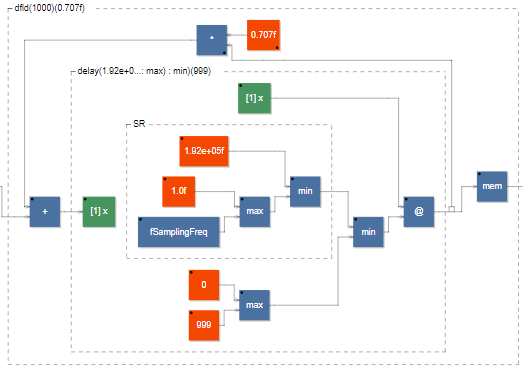
\includegraphics[width=%
0.80\textwidth]{dflfaust}
\caption{delay feedback loop}
\label{fig:dflfaust}
\end{figure}

Il secondo algoritmo derivato permette di realizzare un filtro All Pass, come quello descritto in figura \ref{fig:apf}
\begin{code}
apf(t,g) = _ <: *(-g) + (dfld(t,g)*(1-g^2));
process = os.impulse : apf(1,.71);
\end{code}

Il comportamento All Pass è dato dalla somma del segnale ritardato moltiplicato per $(1-g^2$ e il segnale diretto moltiplicato per $-g$
Il diagramma di questo codice è in figura \ref{fig:apfaust}.

\begin{figure}[htp]
\centering
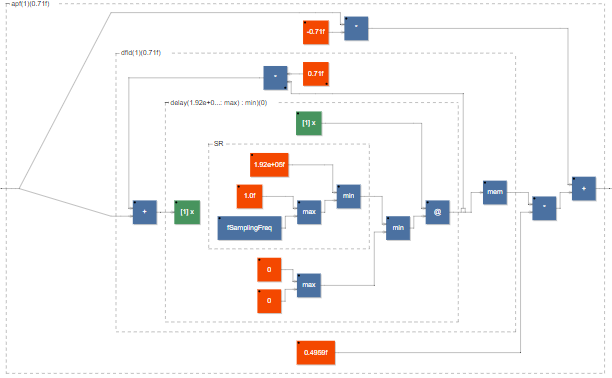
\includegraphics[width=%
0.90\textwidth]{apfaust}
\caption{All Pass}
\label{fig:apfaust}
\end{figure}